
\lecture{Binomial Random Variables}{binomial-random-variables}
\section{Binomial Random Variables}

\title{Binomial Random Variables}
\subtitle{It is either one or the other}

%\author{Kelly Black}
%\institute{Clarkson University}
\date{20 September 2013}

\begin{frame}
  \titlepage
\end{frame}

\begin{frame}
  \frametitle{Outline}
  \tableofcontents[hideothersubsections,sectionstyle=show/hide]
\end{frame}


\subsection{Clicker Quiz}


\iftoggle{clicker}{%
  \begin{frame}
    \frametitle{Clicker Quiz}

    You are going to flip a coin three times. What is the probability of
    getting two tails?

    \vfill

    \begin{tabular}{l@{\hspace{3em}}l@{\hspace{3em}}l@{\hspace{3em}}l}
      A: 1/8 & B: 2/8 & C: 3/8 & D: 4/8
    \end{tabular}

    \vfill
    \vfill
    \vfill


  \end{frame}
}

\subsection{Bernoulli Distribution}


\begin{frame}
  \frametitle{Bernoulli Distribution}

  \begin{definition}
    A random variable is a \redText{Bernoulli distribution} if it has
    a probability mass function that can written in the following form:\\
    \begin{tabular}{r|c}
      X & $p$ \\ \hline
      0 & $1-p$ \\
      1 & $p$
    \end{tabular}
  \end{definition}

\end{frame}


<<<<<<< HEAD
\begin{frame}{Examples}

  \begin{itemize}
  \item Pick a tire at random from a production line: \\
    Report ``1'' if it passes inspection. \\
    Report ``0'' if it does not pass the inspection.
  \item Call a person at random: \\
    Report ``1'' if they support candidate A. \\
    Report ``0'' if they do not support candidate A.

  \end{itemize}
  
=======
  \only<2->{

    \begin{picture}(180,180)
      \put(0,90){\circle*{5}}
      \put(0,90){\line(5,3){50}}
      \put(0,90){\line(5,-3){50}}
      \put(52,120){H}
      \put(52,60){T}

      \only<3->{
        \put(60,130){\line(5,3){40}}
        \put(60,130){\line(5,-2){40}}
        \put(105,157.5){H}
        \put(105,112.5){T}
        \put(60,60){\line(5,2){40}}
        \put(60,60){\line(5,-3){40}}
        \put(105, 67.5){H}
        \put(105, 22.5){T}
      }

      \only<4->{
        \put(115,162.5){\line(5,1){40}}
        \put(115,162.5){\line(5,-1){40}}
        \put(157.5,168.75){H}
        \put(157.5,146.25){T}
        \put(115,117){\line(5,1){40}}
        \put(115,117){\line(5,-1){40}}
        \put(157.5,123.75){H}
        \put(157.5,101.25){T}
        \put(115,74){\line(5,1){40}}
        \put(115,74){\line(5,-1){40}}
        \put(157.5, 78.75){H}
        \put(157.5, 56.25){T}
        \put(115,26){\line(5,1){40}}
        \put(115,26){\line(5,-1){40}}
        \put(157.5, 33.75){H}
        \put(157.5, 11.25){T}
      }

      \only<5->{
        \put(165,173){\line(5,1){20}}
        \put(165,173){\line(5,-1){20}}
        \put(187,177){H}
        \put(187,163){T}

        \put(165,152){\line(5,1){20}}
        \put(165,152){\line(5,-1){20}}
        \put(187,156){H}
        \put(187,142){T}

        \put(165,128){\line(5,1){20}}
        \put(165,128){\line(5,-1){20}}
        \put(187,132){H}
        \put(187,118){T}

        \put(165,107){\line(5,1){20}}
        \put(165,107){\line(5,-1){20}}
        \put(187,111){H}
        \put(187,97){T}

        \put(165,85){\line(5,1){20}}
        \put(165,85){\line(5,-1){20}}
        \put(187,89){H}
        \put(187,75){T}

        \put(165,64){\line(5,1){20}}
        \put(165,64){\line(5,-1){20}}
        \put(187,68){H}
        \put(187,54){T}

        \put(165,37){\line(5,1){20}}
        \put(165,37){\line(5,-1){20}}
        \put(187,41){H}
        \put(187,27){T}

        \put(165,16){\line(5,1){20}}
        \put(165,16){\line(5,-1){20}}
        \put(187,20){H}
        \put(187,6){T}

      }


    \end{picture}

  }


>>>>>>> 7d055f1... Updated the binomial talk
\end{frame}

\begin{frame}{Properties of the Bernoulli Distribution}

  \begin{columns}
    \column{.25\textwidth}
    \begin{tabular}{r|c}
      X & $p$ \\ \hline
      0 & $1-p$ \\
      1 & $p$
    \end{tabular}

    \column{.75\textwidth}
    \begin{eqnarray*}
      E[X] & = & 0\cdot (1-p) + 1\cdot p, \\
      & = & p, \\
      E[X^2] & = & 0^2\cdot (1-p) + 1^2\cdot p, \\
      & = & p, \\
      \mathrm{Var}[X] & = & p - p^2, \\
      & = & p(1-p), \\
      \mathrm{Std.~Dev.} & = & \sqrt{p(1-p)}.
    \end{eqnarray*}
  \end{columns}
\end{frame}

\subsection{Binomial Distribution}

\begin{frame}{Binomial Distribution}

  \begin{itemize}
  \item I have $N$ experiments, $X_1$, $X_2$, $\ldots$, $X_n$.
  \item Each experiment has only two possible outcomes (0/1).
  \item Each experiment has a probability $p$ of a ``1'' outcome.
  \item Each experiment is independent of the others.
  \end{itemize}

  \vfill

  \begin{definition}[Binomial Distribution]
    If $X_1$, $X_2$, $\ldots$, $X_n$ satisfy the conditions above,
    then the random variable
    \begin{eqnarray*}
      X & = & X_1 + X_2 + X_3 + \cdots + X_n
    \end{eqnarray*}
    has a \redText{binomial distribution}.
  \end{definition}

\end{frame}

\begin{frame}{Turn It Around}

 \begin{columns}
    \column{.35\textwidth}

    Flip a coin three times. How many ways to get two tails?

    \column{.65\textwidth}

    \uncover<2->{%

      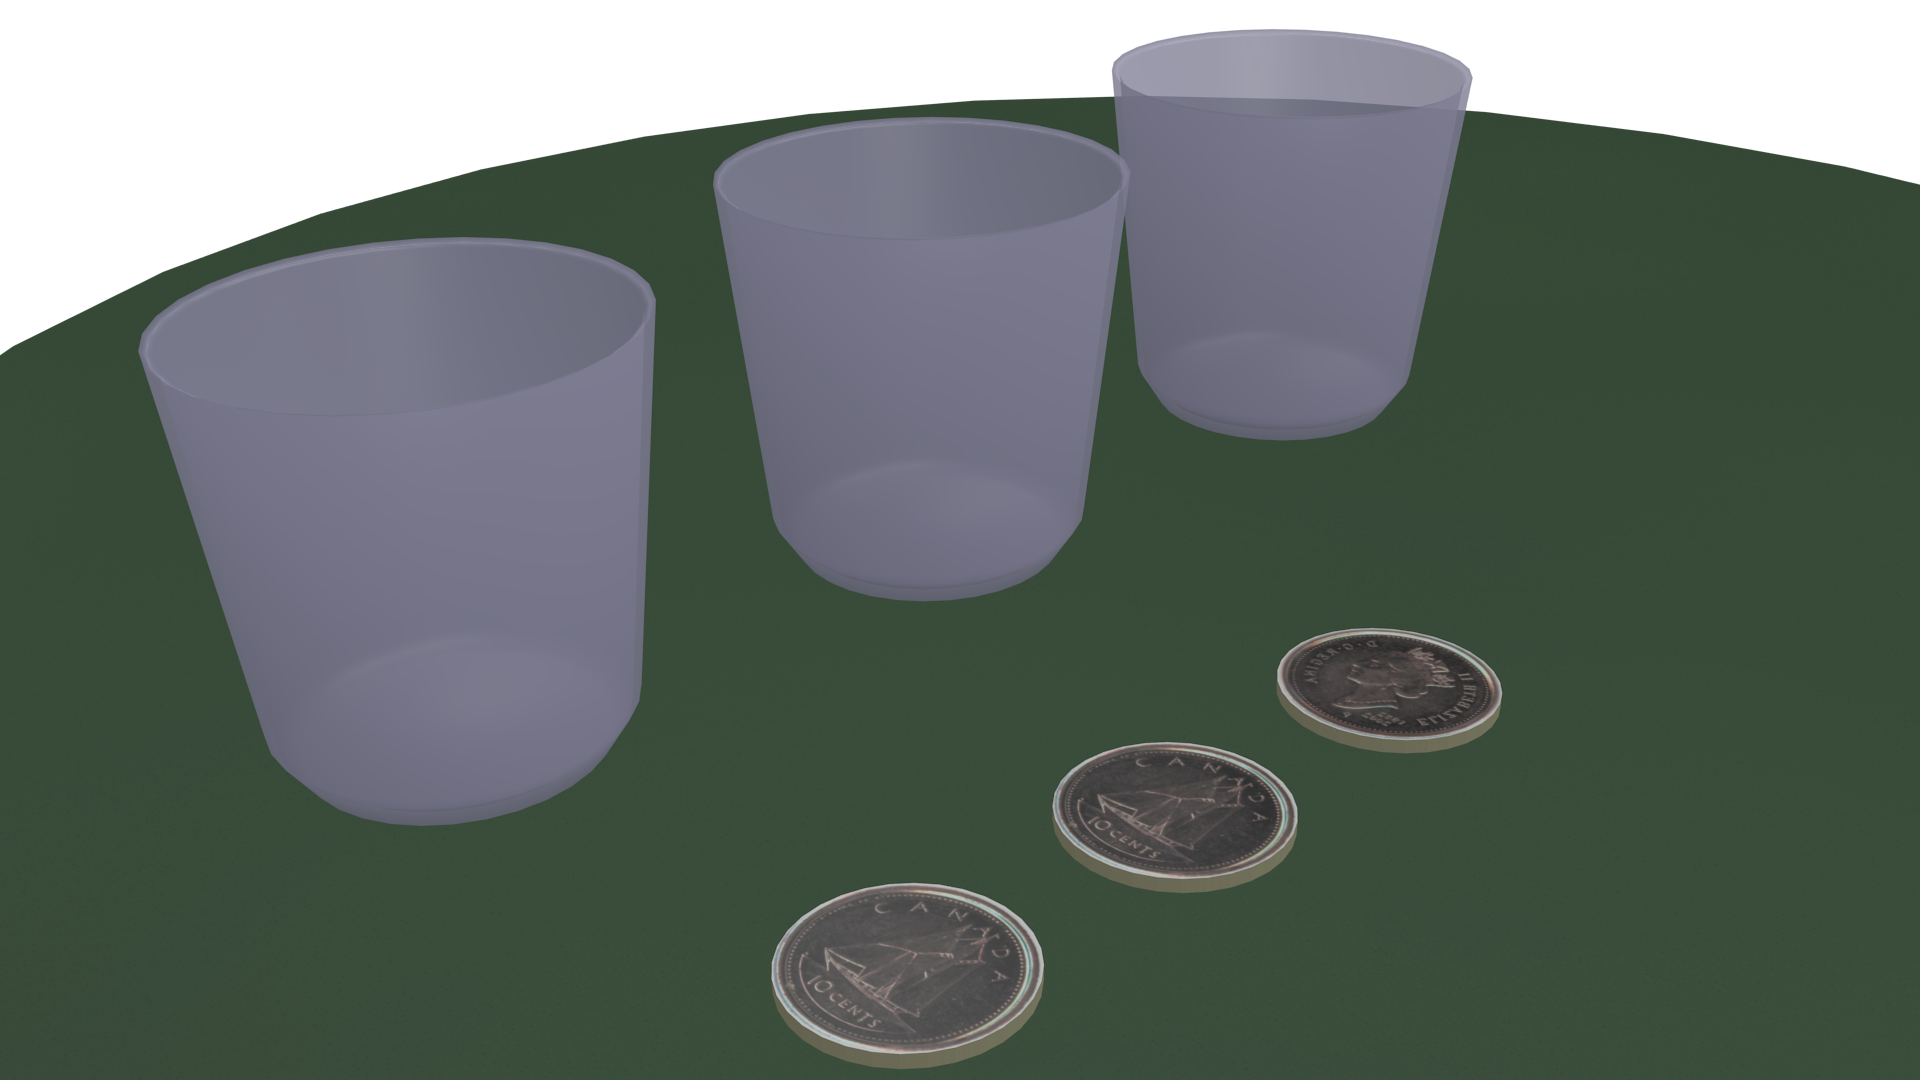
\includegraphics[width=7.5cm]{img/tailsAndCups}

      Change the question: How many ways can I put the tails into three
      cups?
    }

  \end{columns}
  
\end{frame}


\begin{frame}{Binomial Distribution}
    Question: What is the probability of $k$ ``yes'' outcomes?

  \vfill

  In general we have 
  \begin{eqnarray*}
    \underbrace{
      \rule{.3cm}{.2mm} \hspace{.05cm} 
      \rule{.3cm}{.2mm} \hspace{.05cm} 
      \rule{.3cm}{.2mm} \hspace{.05cm} 
      \rule{.3cm}{.2mm} \hspace{.05cm} 
      \rule{.3cm}{.2mm} \hspace{.05cm} \ldots
      \rule{.3cm}{.2mm} \hspace{.05cm} 
      \rule{.3cm}{.2mm} \hspace{.05cm}}_{\mathrm{n~possible~outcomes}}
    & \rightarrow & 
    \underbrace{
      \rule{.3cm}{.2mm} \hspace{.05cm} 
      \rule{.3cm}{.2mm} \hspace{.05cm} 
      \rule{.3cm}{.2mm} \hspace{.05cm} \ldots
      \rule{.3cm}{.2mm} \hspace{.05cm} 
      \rule{.3cm}{.2mm} \hspace{.05cm}}_{\mathrm{k~Yes}}
    \bigg|
    \underbrace{
      \rule{.3cm}{.2mm} \hspace{.05cm} 
      \rule{.3cm}{.2mm} \hspace{.05cm} 
      \rule{.3cm}{.2mm} \hspace{.05cm} \ldots
      \rule{.3cm}{.2mm} \hspace{.05cm} 
      \rule{.3cm}{.2mm} \hspace{.05cm}}_{\mathrm{N-k~No}}
  \end{eqnarray*}

\end{frame}

\begin{frame}{Binomial Distribution}

  In general we have 
  \begin{eqnarray*}
    \underbrace{
      \rule{.3cm}{.2mm} \hspace{.05cm} 
      \rule{.3cm}{.2mm} \hspace{.05cm} 
      \rule{.3cm}{.2mm} \hspace{.05cm} 
      \rule{.3cm}{.2mm} \hspace{.05cm} 
      \rule{.3cm}{.2mm} \hspace{.05cm} \ldots
      \rule{.3cm}{.2mm} \hspace{.05cm} 
      \rule{.3cm}{.2mm} \hspace{.05cm}}_{\mathrm{n~possible~outcomes}}
    & \rightarrow & 
    \underbrace{
      \rule{.3cm}{.2mm} \hspace{.05cm} 
      \rule{.3cm}{.2mm} \hspace{.05cm} 
      \rule{.3cm}{.2mm} \hspace{.05cm} \ldots
      \rule{.3cm}{.2mm} \hspace{.05cm} 
      \rule{.3cm}{.2mm} \hspace{.05cm}}_{\mathrm{k~Yes}}
    \bigg|
    \underbrace{
      \rule{.3cm}{.2mm} \hspace{.05cm} 
      \rule{.3cm}{.2mm} \hspace{.05cm} 
      \rule{.3cm}{.2mm} \hspace{.05cm} \ldots
      \rule{.3cm}{.2mm} \hspace{.05cm} 
      \rule{.3cm}{.2mm} \hspace{.05cm}}_{\mathrm{N-k~No}}
  \end{eqnarray*}

  \vfill

  The probability of this particular outcome is $p^k(1-p)^{N-k}$. 

  \vfill

  There are $\prescript{~}{n}{C}_k$ ways to get $k$ ``yes'' results.
  
  \vfill

  \begin{definition}[Binommial Distribution]
    The probability of $k$ ``yes'' outcomes for a random variable that
    follows a binomial distribution is
    \begin{eqnarray*}
      p(X=k) & = & \prescript{~}{n}{C}_k \cdot p^k (1-p)^{N-k}.
    \end{eqnarray*}
  \end{definition}
  \vfill

  
\end{frame}



\subsection{Examples}

\begin{frame}
  \frametitle{Example}

  I flip a coin ten times. If I report a ``1'' for each tails what is
  the probability of four tails?

  \vfill

\end{frame}


\begin{frame}
  \frametitle{Expectation and Variance}

  $X$ is a random variable with parameters $p$ and $n$.

  \begin{block}{Expectation}
    \begin{eqnarray*}
      E[X] & = & np.
    \end{eqnarray*}
  \end{block}

  \begin{block}{Variation}
    \begin{eqnarray*}
      \mathrm{Var}[X] & = & np(1-p).
    \end{eqnarray*}
  \end{block}

  \begin{block}{Standard Deviation}
    \begin{eqnarray*}
      \mathrm{Standard~Deviation}[X] & = & \sqrt{np(1-p)}.
    \end{eqnarray*}
  \end{block}


\end{frame}

\begin{frame}
  \frametitle{Example}

  I flip a coin ten times. If I report a ``1'' for each tails what is
  the expected value and the standard deviation?

  \vfill

\end{frame}


\iftoggle{clicker}{%
  \begin{frame}{Clicker Quiz}

    A basketball player has a lifetime average of making 70\% of her
    free throws. In a particular game she will attempt eight free
    throws. What is the expected number of free throws that she will
    make?

    \vfill

    \begin{tabular}{l@{\hspace{3em}}l@{\hspace{3em}}l@{\hspace{3em}}l}
      A: 5  & B: 5.6 & C: 6 & D: 8 or we riot!
    \end{tabular}

    \vfill
    \vfill
    \vfill
  
  \end{frame}
}

\begin{frame}{Example}

  Assume that the probability that a plane leaves late from the
  Syracuse airport is 0.12. Assume that this is independent of other
  flights. (Problem!) You plan on taking 14 trips in the upcoming
  year. 

  \begin{itemize}
  \item What is the probability of five late flights?
  \item What is the expected number of late flights?
  \item What is the standard deviation in the number of late flights?
  \end{itemize}
  
\end{frame}

\begin{frame}{Example}

  Forty-eight percent of the people in a district will vote for your
  candidate. You call two-hundred people at random and ask who they
  will vote for. What is the expected number of people who will
  vote your candidate?
  
\end{frame}


% LocalWords:  Clarkson pausesection hideallsubsections
